\documentclass[12pt,a4paper]{article}

\input{../preamble_files/packages}
\input{../preamble_files/figures}
\input{../preamble_files/references}
\input{../preamble_files/shortcuts}
\input{../preamble_files/listings}

\pagestyle{fancy}
\lhead{Richard Whitehill}
\chead{MATH 551 -- HW 2}
\rhead{02/24/22}
\cfoot{\thepage~of~\pageref{LastPage}}

\newcommand{\prob}[2]{\textbf{#1)} #2}

\setlength{\parskip}{\baselineskip}
\setlength{\parindent}{0pt}

\begin{document}

\prob{1}{}

(a) Write the equation for the tangent line to $y = f(x)$ at $x = p$.

$\rightarrow$ The equation of a line passing through $p,f(p)$ with slope $m$ is given as
\begin{align*}
y-f(p) = m(x-p)
\end{align*}
Since the line is tangent to the curve at $x = p$, the slope $m = f'(p)$. Hence,
\begin{align*}
y - f(p) = f'(p)(x-p) \Rightarrow y = f'(p)x + [f(p) - pf'(p)]
\end{align*}

(b) Solve for the $x$-intercept of the line in equation (a).

$\rightarrow$ The $x$-intercept is defined as the value of $x$ such that $y = 0$. We see that
\begin{align*}
0 = f'(p)x + [f(p) - pf'(p)] \Rightarrow x = \frac{pf'(p)-f(p)}{f'(p)} = p - \frac{f(p)}{f'(p)}
\end{align*}
assuming that $f'(p) \not= 0$.

(c) Write the equation for the line that intersects the curve $y = f(x)$ at $x = p$ and $x = q$.

$\rightarrow$ The slope of the line passing through $(p,f(p))$ and $(q,f(q))$ is 
\begin{align*}
m = \frac{f(p)-f(q)}{p-q}
\end{align*}
so we see
\begin{align*}
y - f(p) = \frac{f(p)-f(q)}{p-q}(x-p) \Rightarrow y = \frac{f(p)-f(q)}{p-q}(x-p) + f(p)
\end{align*}

(d) Solve for the $x$-intercept of the line in equation (c).

$\rightarrow$ We can solve for the $x$-intercept for the equation in part (c) as we did for that in part (b):
\begin{align*}
0 &= \frac{f(p)-f(q)}{p-q}(x-p) + f(p) \\
&\frac{f(p)-f(q)}{p-q}(x-p) = -f(p) \\
x-p &= -f(p)\frac{p-q}{f(p)-f(q)} \\
x &= p - \frac{f(p)(p-q)}{f(p)-f(q)}
\end{align*}

\prob{2}{Starting with (0,1), perform two iterations of Newton iteration on the following systems of nonlinear equations
\begin{align*}
\begin{cases}
4x_1^2 - x_2^2 = 0 \\
4x_1x_2^2 - x_1 = 1
\end{cases}
\end{align*}
}

It has been shown that for the system
\begin{align*}
\begin{cases}
f_1(x_1,x_2) = 0 \\
f_2(x_1,x_2) = 0
\end{cases}
\end{align*}
we can find successive approximations to the root as follows:
\begin{align*}
\vec{x}_{n+1} = \vec{x}_{n} - J^{-1}f(\vec{x}_{n})
\end{align*}
where 
\begin{align*}
\vec{x}_n = \begin{pmatrix}
x_{1}^{(n)} \\ x_{2}^{(n)}
\end{pmatrix} 
&\quad
f(\vec{x}_{n}) = \begin{pmatrix}
f_1(x_1^{(n)},x_2^{(n)}) \\ f_2(x_1^{(n)},x_2^{(n)})
\end{pmatrix}
\\
J(x_1,x_2) &= \begin{pmatrix}
\partial f_1/\partial x_1 & \partial f_1/\partial x_2 \\
\partial f_2/\partial x_1 & \partial f_2/\partial x_2
\end{pmatrix}
\end{align*}
For our problem $f_1 = 4x_1^2 - x_2^2$ and $f_2 = 4x_1x_2^2 - x_1 - 1$, so Newton iteration gives
\begin{align*}
\begin{pmatrix}
x_{1}^{(n+1)} \\ x_{2}^{(n+1)}
\end{pmatrix} 
=
\begin{pmatrix}
x_{1}^{(n)} \\ x_{2}^{(n)}
\end{pmatrix} 
-
\begin{pmatrix}
8x_1^{(n)} & -2x_2^{(n)} \\
4(x_2^{(n)})^2 - 1 & 8x_1^{(n)}x_2^{(n)}
\end{pmatrix}^{-1}
\begin{pmatrix}
4(x_1^{(n)})^2 - (x_2^{(n)})^2 \\ 4x_1^{(n)}(x_2^{(n)})^2 - x_1^{(n)} - 1
\end{pmatrix}
\end{align*}
If we begin with $x_1^{(0)} = 0$ and $x_2^{(0)} = 1$, then
\begin{align*}
\begin{pmatrix}
x_{1}^{(1)} \\ x_{2}^{(1)}
\end{pmatrix} 
=
\begin{pmatrix}
0 \\ 1
\end{pmatrix} 
-
\begin{pmatrix}
0 & -2 \\
3 & 0
\end{pmatrix}^{-1}
\begin{pmatrix}
-1 \\ -1
\end{pmatrix}
=
\begin{pmatrix}
0 \\ 1
\end{pmatrix} 
-
\begin{pmatrix}
-1/3 \\ 1/2
\end{pmatrix} 
=
\begin{pmatrix}
1/3 \\ 1/2
\end{pmatrix}
\end{align*}
Repeating for a second time we see
\begin{align*}
\begin{pmatrix}
x_{1}^{(2)} \\ x_{2}^{(2)}
\end{pmatrix} 
=
\begin{pmatrix}
1/3 \\ 1/2
\end{pmatrix} 
-
\begin{pmatrix}
8/3 & -1 \\
0 & 4/3
\end{pmatrix}^{-1}
\begin{pmatrix}
7/36 \\ -1
\end{pmatrix}
=
\begin{pmatrix}
1/3 \\ 1/2
\end{pmatrix} 
-
\begin{pmatrix}
-5/24 \\ -3/4
\end{pmatrix} 
=
\begin{pmatrix}
13/24 \\ 5/4
\end{pmatrix}
\end{align*}

\prob{3}{Write a program to compute the square root of $m$ by bisection method when $m = 7,~13,~17$. The interval $[a,b]$ where the square root is located is $[s,s+1]$, where $s$ is an integer and $s^2 < m < (s+1)^2$. Please find the approximate solution with 7 iteration steps, i.e. find $c_0,c_1,\hdots,c_7$.}

$\rightarrow$ The bisection method program is shown below and gives the following results after 7 iteration steps.
\begin{table}[H]
\begin{center}
\begin{tabular}{c|c|c}
$m$ & $s$ & $\sqrt{m}$ \\
\hline
7 & 2 & 2.644531 \\
13 & 3 & 3.605469 \\
17 & 4 & 4.121094 \\
\end{tabular}
\end{center}
\end{table}

An image of the program output is displayed below to demonstrate the successive approximations:
\bef
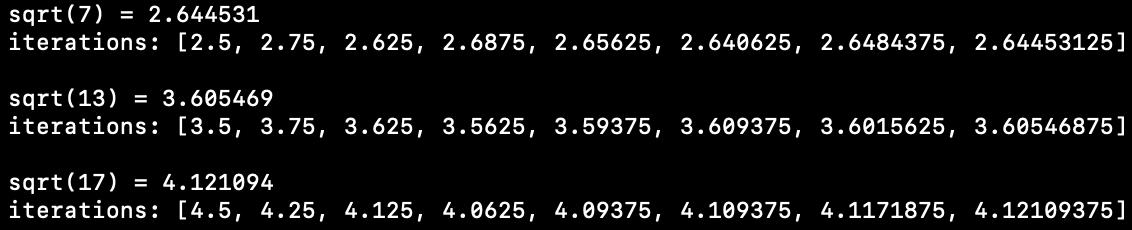
\includegraphics[scale=0.75]{fig1.png}
\eef

\inputpython{./prob3.py}

\prob{4}{Find the root of $f(x) = x^2 - 3$ by Newton's method, with initial guess $x_0 = -100,-5,$ $-0.001,0,0.001,5,100$. Discuss your findings.}

$\rightarrow$ The results of the program which computes the answers for each initial guess using Newton's method is shown below and the results are shown in the table below and in the figure of the program output below. It is seen that the results are similar in magnitude. Notice that when the initial guess and the root have the same sign, which is expected since the function is convex if restrict our domain to either $\reals^{-}$ or $\reals^{+}$ with a range $\reals^{+}$, which guarantees that the algorithm converges to the simple root on the domain. Trivially, it is also observed that an initial guess of $x_0 = 0$ gives an error since $f'(0) = 0$
\begin{table}[H]
\begin{center}
\begin{tabular}{c|c}
$x_0$ & root \\
\hline
-100 & -1.73205 \\
-5 & -1.73205 \\
-0.001 & -1.73205 \\
0 & Error \\
0.001 & 1.73205 \\
5 & 1.73205 \\
100 & 1.73205 
\end{tabular}
\end{center}
\end{table}
\bef
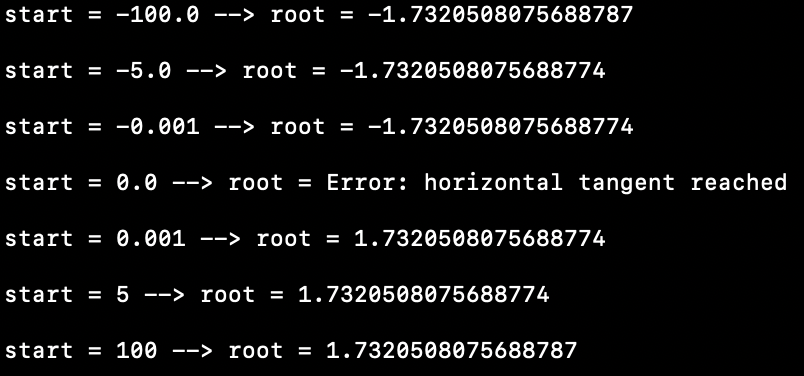
\includegraphics[scale=0.75]{fig2.png}
\eef

\inputpython{./prob4.py}

\prob{5}{Write down the first three iterations of the secant method for solving $x^2-3 = 0$, starting with $x_0=0$ and $x_1 = 1$. Meanwhile, programming with MATLAB to obtain approximation accurate within $10^{-6}$.}

The secant method follows an iterative algorithm defined by the recursion relation
\begin{align*}
x_{n+1} = x_n - f(x_n)\frac{x_n - x_{n-1}}{f(x_n) - f(x_{n+1})}
\end{align*} 
Thus, if $f(x) = x^2-3$, $x_0 = 0$, and $x_1 = 1$, then
\begin{align*}
x_2 &= 1 - (-2)\frac{1-0}{-2-(-3)} = 3 \\
x_3 &= 3 - (6)\frac{3-1}{6-(-2)} = \frac{3}{2} \\
x_4 &= \frac{3}{2} - \left(-\frac{3}{4}\right)\frac{3/2 - 3}{-3/4 - 6} = \frac{5}{3} = 1.\bar{6}
\end{align*}
Using a computer to obtain an approximation accurate to the sixth decimal place: 1.732051. Below are the figure showing the output of the program and the code used to implement the secant method.

\bef

\includegraphics[scale=1]{fig3.png}
\eef

\inputpython{./prob5.py}

\end{document}
